\pagenumbering{arabic}
%\documentclass[slides]{beamer}
\documentclass[mathserif,8pt]{beamer}
%\documentclass[slides,hyperref={pdfpagelabels=false}]{beamer}
%\documentclass[handout,gray]{beamer}
\usepackage[T1]{fontenc}
\usepackage[utf8]{inputenc}
\usepackage{textcomp}
\usepackage{verbatim}
\usepackage{amsbsy}
\usepackage{multicol}
\usepackage{booktabs} % Make some nice tables
\usepackage{ae,aecompl}

%%%%%%%%%%%% COULEURS %%%%%%%%%%%%%%%%%%%%%%%%%%%

\mode<presentation>
{
  \definecolor{beamerstructure}{RGB}{43,79,112}
  \definecolor{sidebackground}{RGB}{230,242,250}
  \definecolor{CTCC}{RGB}{133,188,228}
  \color{beamerstructure}
  \usetheme{default}
  \usepackage{courier}
  \beamertemplateballitem
\setbeamertemplate{navigation symbols}{}
%\setbeamertemplate{sidebar left}{\thispdfpagelabel{\insertframenumber}}
%\setbeamertemplate{footline}{\quad\insertframenumber}
%\usecolortheme{CTCC}
}
\usebackgroundtemplate{\includegraphics[width=1.02\paperwidth]{../templets/ctcc_general.jpg}}

\title{\\\vspace{1cm} Relativistic effects in chemistry}
%\subtitle{\textcolor{magenta}{My subtitle (if applicable)}}
\author{Stig Rune Jensen}
\institute[CTCC]{\\[-6mm]stig.r.jensen@uit.no\\[6mm]UiT The Arctic University of Norway\\[6mm]
\includegraphics[height=1.5cm]{../templets/uio.pdf}\hspace{1cm} 
\includegraphics[height=1.5cm]{../templets/sff.pdf}\hspace{1cm}
\includegraphics[height=1.5cm]{../templets/uit.pdf}}
\date{Troms\o, March 20th 2014}

\newcommand{\gb}[1]{green!#1!black}
\newcommand{\rb}[1]{red!#1!black}
\newcommand{\bb}[1]{blue!#1!black}
\newcommand{\coleq}{red!60!black}
\newcommand{\du}{\textrm{d}}

\usepackage{multicol}
\newcommand{\mydef}{\stackrel{\text{def}}{\hbox{=}}} 

\begin{document}

\footnotesize
\setlength{\unitlength}{\textwidth}

{
\usebackgroundtemplate{\includegraphics[width=1.02\paperwidth]{../templets/ctcc_forside.jpg}}
\maketitle
}

\begin{frame}
    \frametitle{Relativistic effects in chemistry}
    \begin{columns}
    \begin{column}{.7\textwidth}
	\centering
	\begin{exampleblock}{{\it{''These [relativistic effects] give rise to difficulties 
	    only when high-speed particles are involved, and are therefore of \textcolor{red}{no 
	    importance} in the consideration of atomic and molecular structure and ordinary 
	    chemical reactions\dots''}}}
	    \vskip2mm
	    \hspace*\fill{\tiny--- Paul AM Dirac, 1929}
	\end{exampleblock}
    \end{column}
    \begin{column}{.3\textwidth}
	\centering
	\includegraphics[viewport = 50 200 500 800, clip, scale=0.15]{figures/dirac.pdf}
    \end{column}
    \end{columns}
    \ \\
    \ \\
    \ \\
    \ \\
    \ \\
    \ \\
    \pause
    \centering
    \textbf{Speed of core electrons}
    \begin{equation}
	\nonumber
	v \approx \frac{Z}{137}c
    \end{equation}
\end{frame}

\begin{frame}
    \frametitle{Physical theories}
    \begin{columns}
    \begin{column}{.30\textwidth}
	\centering
	\textbf{Sir Isaac Newton}\\
	\includegraphics[viewport = 50 400 360 800, clip, scale=0.15]{figures/newton.pdf}
    \end{column}
    \begin{column}{.40\textwidth}
    \ \ \ \ \textbf{Newtonian mechanics}
    \begin{itemize}
	\item Sir Isaac Newton (1687)
	\item valid at ''normal'' length scales
	\item valid for slow moving objects ($v \ll c$)
    \end{itemize}
    \end{column}
    \begin{column}{.30\textwidth}
	\centering
	\textbf{Erwin Schr\"{o}dinger}\\
	\includegraphics[viewport = 100 400 370 800, clip, scale=0.15]{figures/schrodinger.pdf}
    \end{column}
    \end{columns}
    \ \\
    \ \\
    \ \\
    \begin{columns}
    \begin{column}{.15\textwidth}
	\ \\
    \end{column}
    \begin{column}{.35\textwidth}
    \ \ \ \ \textbf{Special relativity}
    \begin{itemize}
	\item Albert Einstein (1905)
	\item valid at ''normal'' length scales
	\item valid for all velocities ($v \leq c$)
    \end{itemize}
    \end{column}
    \begin{column}{.35\textwidth}
    \ \ \ \ \textbf{Quantum mechanics}
    \begin{itemize}
	\item Erwin Schr\"{o}dinger (1926)
	\item valid at small length scales
	\item valid for low velocities ($v \ll c$)
    \end{itemize}
    \end{column}
    \begin{column}{.15\textwidth}
	\ \\
    \end{column}
    \end{columns}
    \ \\
    \ \\
    \ \\
    \begin{columns}
    \begin{column}{.30\textwidth}
	\centering
	\textbf{Albert Einstein}\\
	\includegraphics[viewport = 50 200 500 800, clip, scale=0.1]{figures/einstein.pdf}
    \end{column}
    \begin{column}{.40\textwidth}
    \ \ \ \ \textbf{Relativistivc quantum mechanics}
    \begin{itemize}
	\item Paul AM Dirac (1928)
	\item valid at small length scales
	\item valid for all velocities ($v \leq c$)
    \end{itemize}
    \end{column}
    \begin{column}{.30\textwidth}
	\centering
	\textbf{Paul AM Dirac}\\
	\includegraphics[viewport = 50 200 500 800, clip, scale=0.1]{figures/dirac.pdf}
    \end{column}
    \end{columns}
\end{frame}

\begin{frame}
    \frametitle{Theory of special relativity}
    \begin{columns}
    \begin{column}{.60\textwidth}
	\centering
	\begin{exampleblock}{\it{\small{''Henceforth space by itself, and time by itself,
	    are doomed to fade away into mere shadows, and only a kind of union of the
	    two will perserve an independent reality.''}}}
	    \vskip2mm
	    \hspace*\fill{\tiny--- Hermann Minkowski}
	\end{exampleblock}
    \end{column}
    \begin{column}{.40\textwidth}
	\centering
	\includegraphics[viewport = 70 600 270 780, clip, scale=0.4]{figures/minkowski.pdf}
    \end{column}
    \end{columns}
    \ \\
    \ \\
    \ \\
    \ \\
    \ \\
    \begin{columns}
    \begin{column}{.30\textwidth}
    \ \ \ \ \textbf{Newtonian mechanics}
    \begin{itemize}
	\item \textbf{Absolute} space and time
	\item \textbf{Separates} space and time
	\item Galilean transformations\\
	    \begin{align}
		\nonumber
		x' &= x - vt\\
		\nonumber
		t' &= t
	    \end{align}
    \end{itemize}
    \end{column}
    \begin{column}{.40\textwidth}
	\centering
	\includegraphics[viewport = 50 550 430 800, clip, scale=0.3]{figures/reference_frame.pdf}
    \end{column}
    \begin{column}{.30\textwidth}
    \ \ \ \ \textbf{Relativistic mechanics}
    \begin{itemize}
	\item \textbf{Relative} space and time
	\item \textbf{Mixes} space and time
	\item Lorentz transformations\\
	    \begin{align}
		\nonumber
		x' &= \gamma (x - vt)\\
		\nonumber
		t' &= \gamma (t - vx/c^2)
	    \end{align}
    \end{itemize}
    \end{column}
    \end{columns}
\end{frame}

\begin{frame}
    \frametitle{Theory of special relativity}
    \begin{columns}
    \begin{column}{.60\textwidth}
	\begin{itemize}
	\item Lorentz factor
	\begin{equation}
	    \nonumber
	    \gamma = \frac{1}{\sqrt{1-v^2/c^2}}
	\end{equation}
	\ \\
	\ \\
	\ \\
	\item The speed of light is the same in all reference frames\\
	\ \\
	\ \\
	\item $c$ remains constant as space and time themselves change\\
	\ \\
	\ \\
	\item Implications are often paradoxical and counter intuitive\\
	\ \\
	\ \\
	\item Nothing (particles or information) can move faster\\ than the speed of light\\
	\end{itemize}
	\ \\
	\ \\
	\ \\
	\ \\
	\centering
	\includegraphics[viewport = 60 710 210 780, clip, scale=0.5]{figures/speed_limit.pdf}
    \end{column}
    \begin{column}{.40\textwidth}
	\centering
	\includegraphics[viewport = 100 400 550 750, clip, scale=0.25]{figures/lorentz_factor.pdf}\\
	\ \\
	\ \\
	\ \\
	\ \\
	\ \\
	\ \\
	\includegraphics[viewport = 70 550 390 770, clip, scale=0.3]{figures/light_beam.pdf}
	\ \\
    \end{column}
    \end{columns}
\end{frame}

\begin{frame}
    \frametitle{Relativistic effects in physics}
    \begin{columns}
    \begin{column}{.30\textwidth}
    \begin{itemize}
	\item \textbf{Mass increase}
	    \begin{equation}
		\nonumber
		m_{rel} = \gamma m_0
	    \end{equation}
	\ \\
	\ \\
	\ \\
	\item \textbf{Length contraction}
	    \begin{equation}
		\nonumber
		x_{rel} = \frac{x_0}{\gamma}
	    \end{equation}
	\ \\
	\ \\
	\ \\
	\item \textbf{Time dilation}
	    \begin{equation}
		\nonumber
		t_{rel} = \gamma t_0
	    \end{equation}
	\ \\
	\ \\
	\ \\
	\item \textbf{Simultaneity is relative}
    \end{itemize}
    \end{column}
    \begin{column}{.70\textwidth}
	\centering
	\ \\
	\ \\
	\ \\
	\ \\
	\includegraphics[viewport = 100 400 520 760, clip, scale=0.4]{figures/mass_and_energy.pdf}\\
    \end{column}
    \end{columns}
\end{frame}

\begin{frame}
    \frametitle{Relativistic effects in physics}
    \textbf{What are relativistic effects and how can we study them?}\\
    \ \\
    \begin{itemize}
        \item	Nature is \textbf{relativistic} so non-relativistic experiments are not possible
        \item	Non-relativistic limit obtained \textbf{theoretically} by letting $c\rightarrow\infty$.
        \item	Relativistic effects are the differences between the full relativistic theory and
		the non-relativistic limit
        \item	Example: The Maxwell equations
    \end{itemize}
    \ \\
    \ \\
    \ \\
    \ \\
    \pause
    \begin{columns}
    \begin{column}{.10\textwidth}
	\ \\
    \end{column}
    \begin{column}{.35\textwidth}
	\centering
	\ \ \ \textbf{Relativistic}
	\begin{align}
	    \nonumber
	    \nabla \cdot  \boldsymbol{B} &= 0\\
	    \nonumber
	    \nabla \times \boldsymbol{E} + \frac{\partial \boldsymbol{B}}{\partial t} &= 0\\
	    \nonumber
	    \nabla \cdot  \boldsymbol{E} &= \frac{\rho}{\epsilon_0}\\
	    \nonumber
	    \nabla \times \boldsymbol{B} - \frac{1}{c^2}\frac{\partial \boldsymbol{E}}{\partial t} &= 
		\frac{1}{\epsilon_0 c^2} \boldsymbol{j}
	\end{align}
    \end{column}
    \pause
    \begin{column}{.35\textwidth}
	\centering
	\ \ \ \ \textbf{Non-relativistic}
	\begin{align}
	    \nonumber
	    \nabla \cdot  \boldsymbol{B} &= 0\\
	    \nonumber
	    \nabla \times \boldsymbol{E} + \frac{\partial \boldsymbol{B}}{\partial t} &= 0\\
	    \nonumber
	    \nabla \cdot  \boldsymbol{E} &= \frac{\rho}{\epsilon_0}\\
	    \nonumber
	    \nabla \times \boldsymbol{B} &= 0
	\end{align}
	\ \\
	\ \\
    \end{column}
    \begin{column}{.20\textwidth}
	\ \\
    \end{column}
    \end{columns}
    \ \\
    \ \\
    \ \\
    \pause
    \centering
    \textbf{Magnetic fields is a relativistic effect!}
\end{frame}

\begin{frame}
    \frametitle{Quantum mechanics}
    \begin{columns}
    \begin{column}{.50\textwidth}
	\centering
	Electrons influenced by a nuclear potential $V_n$\\
	are described by the time-independent equation
	\begin{equation}
	    \nonumber
	    \hat{H} \psi = E \psi
	\end{equation}
	\ \\
	\ \\
	with one- and two-particle terms
	\begin{equation}
	    \nonumber
	    \hat{H} = \sum_i h_i + \sum_{i<j} g_{ij}
	\end{equation}
    \end{column}
    \begin{column}{.4\textwidth}
	\ \\
	\ \\
	\ \ \ \ \textbf{Non-relativistic theory}
	\begin{itemize}
	    \item Schr\"{o}dinger one-particle Hamiltonian
	    \begin{equation}
		\nonumber
		h_i^{NR}  = \left[\frac{\boldsymbol{p}^2}{2m} + V_n\right]
	    \end{equation}
	    \item two-particle Coulomb interaction
	    \begin{equation}
		\nonumber
		g_{ij}^C = \frac{1}{r_{ij}} 
	    \end{equation}
	\end{itemize}
    \end{column}
    \begin{column}{.1\textwidth}
	\ \\
    \end{column}
    \end{columns}
    \ \\
    \ \\
    \ \\
    \pause
    \begin{columns}
    \begin{column}{.45\textwidth}
	\ \ \ \ \textbf{Relativistic theory}
	\begin{itemize}
	    \item Dirac one-particle Hamiltonian
		\begin{equation}
		    \nonumber
		    h_i^R = \begin{bmatrix}
			\left(mc^2 + V_n\right) & c\boldsymbol{\sigma}\cdot\boldsymbol{p}\\
			c\boldsymbol{\sigma}\cdot\boldsymbol{p}&-\left(mc^2 + V_n\right)\\
			    \end{bmatrix}
		\end{equation}
	    \item where $\boldsymbol{\sigma}$ are the Pauli spin matrices ($2\times2$)
	\end{itemize}
    \end{column}
    \begin{column}{.55\textwidth}
	\ \\
	\ \\
	\ \\
	\ \\
	\begin{itemize}
	    \item we thus get a four-component wave function
		\begin{equation}
		    \nonumber
		    \psi^{R} =	\begin{bmatrix}
				\psi_\alpha^L,\psi_\beta^L,\psi_\alpha^S,\psi_\beta^S
				\end{bmatrix}
		\end{equation}
	    \item   the two-particle interaction is no longer exact,\\
		    and we have the Coulomb-Breit approximation
		\begin{equation}
		    \nonumber
		    g_{ij}^{CB} = \frac{1}{r_{ij}} - 
		    \frac{\boldsymbol{\alpha}_i\cdot \boldsymbol{\alpha}_j}{r_{ij}} -
		    \frac{(\boldsymbol{\alpha}_i\cdot \boldsymbol{r}_{ij})
		    (\boldsymbol{\alpha}_j\cdot \boldsymbol{r}_{ij})}{r_{ij}^3} + \cdots
		\end{equation}
	\end{itemize}
    \end{column}
    \end{columns}
\end{frame}

\begin{frame}
    \frametitle{Relativistic free particle}
    \begin{columns}
    \begin{column}{.40\textwidth}
	\centering
	\textbf{Free particle energy}
        \begin{equation}
	   \nonumber
	   E = \pm \sqrt{p^2c^2+m^2c^4}
	\end{equation}
	\ \\
	\ \\
	\ \\
	\begin{itemize}
	    \item   there are negative energy states\\
	    \ \\
	    \item   in the vacuum reference all negative\\ 
		    energy states are filled (Dirac sea)\\
	    \ \\
	    \item   exitation across the $\Delta E = 2mc^2$ energy\\
		    barrier creates \textbf{electron-positron pair}
	\end{itemize}
    \end{column}
    \begin{column}{.60\textwidth}
	\centering
	\only<1>{\ \ \ \includegraphics[viewport = 100 420 520 750, clip, scale=0.3]{figures/electron_positron_1.pdf}}
	\only<2>{\ \includegraphics[viewport = 100 420 520 750, clip, scale=0.3]{figures/electron_positron_2.pdf}}
	\only<3>{\includegraphics[viewport = 100 420 520 750, clip, scale=0.3]{figures/electron_positron_3.pdf}}
    \end{column}
    \end{columns}
\end{frame}

\begin{frame}
    \frametitle{Approximate Hamiltonians}
    \begin{columns}
    \begin{column}{.75\textwidth}
    \textbf{The full four-component Dirac Hamiltonian can be approximated in several ways}\\
    \ \\
    \begin{itemize}
	\item	it can be decoupled by a unitary transformation into two-component form
		\begin{equation}
		    \nonumber
		    U^\dag h^RU = \begin{bmatrix}h_+&0\\0&h_-\\ \end{bmatrix}
		\end{equation}
		\ \\
		\ \\
	\item	or we can start from a \textbf{non-relativistic} wave function and treat relativistic\\
		effects as a \textbf{perturbation}, in which case we get the Pauli Hamiltonian
		\begin{equation}
		    \nonumber
		    H^{pauli} = h^{NR} + h^{mv} + h^{darwin} + h^{so} + \cdots
		\end{equation}
		\ \\
		\ \\
	\item	where the corrections are separated into \textbf{scalar relativistic effects}
		\begin{equation}
		    \nonumber
		    h^{mv} = -\frac{p^4}{8m^3c^2}, \qquad\qquad\qquad
		    h^{darwin} = \frac{1}{8m^2c^2} \nabla^2V
		\end{equation}
		\ \\
		\ \\
	\item	and \textbf{spin-orbit effects}
		\begin{equation}
		    \nonumber
		    h^{so} = \frac{1}{4m^2c^2}\boldsymbol{\sigma}\cdot
		    \left[\left(\nabla V\right)\times\boldsymbol{p}\right]
		\end{equation}
    \end{itemize}
    \end{column}
    \begin{column}{.25\textwidth}
	\ \\
    \end{column}
    \end{columns}
\end{frame}

\begin{frame}
    \frametitle{Scalar relativistic effects}
    \begin{itemize}
	\item	Electron speed related to nuclear charge $Z$
		and principal quantum number $n$
		\begin{equation}
		    \nonumber
		    \frac{v_e}{c} \approx \frac{Z}{n\alpha},\qquad \alpha \approx 137
		\end{equation}
		\ \\
		\ \\
		\ \\
	\item	giving an \textbf{increase} in electron mass
		\begin{equation}
		    \nonumber
		    m_{rel} = \gamma m_e \approx \frac{m_e}{\sqrt{1-Z^2/(n\alpha)^2}}
		\end{equation}
		\ \\
		\ \\
		\ \\
	\item	\textbf{contraction} of the Bohr radius
		\begin{equation}
		    \nonumber
		    a_{rel} = \frac{a_0}{\gamma} \approx a_0\sqrt{1-Z^2/(n\alpha)^2}
		\end{equation}
		\ \\
		\ \\
		\ \\
	\item	and the \textbf{mass-velocity} energy correction
		\begin{equation}
		    \nonumber
		    h^{mv} = -\frac{p^4}{8m^3c^2}
		\end{equation}
		\ \\
		\ \\
		\ \\
	\item	Relativity leads to \textbf{orbital contraction} and a \textbf{lowering} of the energy, 
		and the effect\\ is greater with higher nuclear charge and lower principal quantum number
    \end{itemize}
\end{frame}

\begin{frame}
    \frametitle{Scalar relativistic effects}
    \ \\
    \begin{columns}
    \begin{column}{.50\textwidth}
    \centering
    \textbf{The Darwin energy correction}
    \begin{equation}
	\nonumber
	h^{darwin} = \frac{1}{8m^2c^2} \nabla^2 V
    \end{equation}
    \ \\
    \ \\
    \ \\
    \ \\
    \ \\
    \begin{itemize}
	\item Originates from ''zitterbewegung''\\
	\ \\
	\item Energy from oscillatory motion of the electron\\
	\ \\
	\item Similar to classical Brownian motion where the absolute speed
	of the particle is higher than its average velocity\\
	\ \\
	\item Contiuous creation and annihilation of electron-positron pairs
    \end{itemize}
    \ \\
    \end{column}
    \begin{column}{.50\textwidth}
	\centering
	\includegraphics[viewport = 60 450 500 800, clip, scale=0.25]{figures/brownian_motion.pdf}\\
	\includegraphics[viewport = 0 0 300 300, clip, scale=0.3]{figures/zitterbewegung.pdf}
    \end{column}
    \end{columns}
\end{frame}

\begin{frame}
    \frametitle{Spin-orbit effects}
    \begin{columns}
    \begin{column}{.10\textwidth}
	\ \\
    \end{column}
    \begin{column}{.40\textwidth}
	\centering
    \textbf{General expression}
    \begin{equation}
	\nonumber
	h^{so} = \frac{1}{4m^2c^2}\boldsymbol{\sigma}\cdot
	    \left[\left(\nabla V\right)\times\boldsymbol{p}\right]
    \end{equation}
    \end{column}
    \begin{column}{.40\textwidth}
	\centering
	\textbf{Spherical potential ($V=Z/r$)}
	\begin{equation}
	    \nonumber
	    h^{so} = \frac{Z}{c^2}\frac{\boldsymbol{s}\cdot\boldsymbol{l}}{r^3}
	\end{equation}
    \end{column}
    \begin{column}{.10\textwidth}
	\ \\
    \end{column}
    \end{columns}
    \ \\
    \ \\
    \ \\
    \ \\
    \begin{columns}
    \begin{column}{.40\textwidth}
    \begin{itemize}
	\item	a particle \textbf{moving} in an electric field will see a \textbf{magnetic field}\\
		\ \\
	\item	this is a \textbf{relativistic effect}, an element of a Lorentz transformation\\
		\ \\
	\item	SO is a \textbf{magnetic interaction} between the electron magnetic moment\\ 
		(spin) and the magnetic field due to the relative motion of the charges\\
		\ \\
	\item	allows \textbf{spin forbidden transitions} (phosphorescence)\\
		\ \\
	\item	responsible for the \textbf{fine structure splitting} of atomic spectral lines
    \end{itemize}
    \end{column}
    \begin{column}{.40\textwidth}
	\includegraphics[viewport = 230 230 380 400, clip, scale=0.8]{figures/phosphorescence.pdf}
    \end{column}
    \end{columns}
\end{frame}

%\begin{frame}
    %\frametitle{Relativistic computational chemistry}
    %\begin{columns}
    %\begin{column}{.50\textwidth}
    %\textbf{How complete is the theory?}
    %\begin{itemize}
	%\item Quantum Electrodynamics (QED)
	%\item Self-Energy and  Vacuum Polarization ($<1\%$)
	%\item Finite vs. point nucleus (comparable for high $Z$)
	%\item Parity non-conservation
	%\item Retardation effects
    %\end{itemize}
    %\ \\
    %\ \\
    %\ \\
    %\textbf{How accurately can we do calculations?}
    %\begin{itemize}
	%\item Full 4-component (Dirac-Coulomb-Breit)
	%\item Approximate 2-component (Douglas-Kroll-Hess)
	%\item Perturbative 1-component (Breit-Pauli)
	%\item Pseudopotentials (effective core potentials)
	%\item Electron correlation
	%\item Basis set
    %\end{itemize}
    %\end{column}
    %\begin{column}{.50\textwidth}
	%\centering
	%\includegraphics[viewport = 100 400 600 800, clip, scale=0.35]{figures/relativistic_accuracy.pdf}
    %\end{column}
    %\end{columns}
%\end{frame}

\begin{frame}
    \frametitle{Relativistic atomic structure}
    \begin{columns}
    \begin{column}{.50\textwidth}
	\centering
    	\textbf{Energy of hydrogenic ion}
	\begin{equation}
	    \nonumber
	    E = -\frac{Z^2}{2n^2} + \frac{Z^4}{2n^4c^2}\left(\frac{3}{4}-\frac{n}{j+1/2}\right) + \cdots
	\end{equation}
	\ \\
	\ \\
	\ \\
	\begin{itemize}
	    \item   Spin-orbit splitting of energy levels 
	    \item   Strong dependence on atomic number\\ 
		    for hydrogenic ions ($Z^4$)
	    \item   Weaker dependence for valence shells\\
		    in many-electron atoms ($Z^2$)
	    \item   Orbital angular momentum $l$ and spin $m_s$\\
		    quantum numbers no longer appropriate
	    \item   Total angular momentum $j$ is\\
		    the proper quantum number
	    \item   Orbital symmetry depends on $j$ rather\\ 
		    than $l$ (\textbf{s$_{1/2}$ and p$_{1/2}$ are both spherical})
	\end{itemize}
    \end{column}
    \begin{column}{.50\textwidth}
	\centering
	\includegraphics[viewport = 50 450 530 780, clip, scale=0.3]{figures/spin_orbit_splitting.pdf}\\
	\ \\
	\ \\
	\ \\
	\includegraphics[viewport = 120 535 470 685, clip, scale=0.4, angle=-2]{figures/relativistic_orbitals.pdf}
    \end{column}
    \end{columns}
\end{frame}

\begin{frame}
    \frametitle{The periodic table}
    \begin{columns}
    \begin{column}{.45\textwidth}
	\textbf{Scalar relativistic effects}
	\ \\
	\ \\
	\begin{itemize}
	    \item   increases as $Z^2$ for valence electrons
	    \item   \textbf{contraction} of s- and p-shells
	    \item   \textbf{indirect expansion} of d- and f-shells
	    \item   often explain the differences between\\ 
		    the 5th and 6th row elements
	    \item   \textbf{lanthanide contraction} ($Z=58\rightarrow71$)
	    \item   \textbf{theoretical} periodic table available\\
		    up to element ($Z=172$)\\
		    \scriptsize{\it{Phys. Chem. Chem. Phys.}, 2011, \textbf{13}, 161}
	\end{itemize}
    \end{column}
    \begin{column}{.55\textwidth}
	\centering
	\includegraphics[viewport = 0 500 550 800, clip, scale=0.3]{figures/periodic_table.pdf}\\
	\includegraphics[viewport = 0 520 520 800, clip, scale=0.3]{figures/orbital_energies.pdf}
    \end{column}
    \end{columns}
\end{frame}

\begin{frame}
    \frametitle{The gold atom}
    \begin{columns}
    \begin{column}{.55\textwidth}
	\textbf{Relativistic effects reaches a maximum at gold ($Z=79$)}\\
	\ \\
	\begin{itemize}
	    \item   1s electron moves at 58\% of the speed of light
	    \item   1s orbital contracts by 22\%
	    \item   color originates from the $(n-1)d$ to $ns$ transition
	    \item   \textbf{without relativity gold and silver would be similar}
	    \item   relativity accounts for most of the differences\\
		    between gold and mercury ($Z=80$)
	\end{itemize}
	\centering
	\includegraphics[viewport = 50 50 350 300, clip, scale=0.4]{figures/gold_energy.pdf}
    \end{column}
    \begin{column}{.45\textwidth}
	\centering
	\includegraphics[viewport = 50 580 380 780, clip, scale=0.4]{figures/gold_maximum.pdf}\\
	\ \\
	\ \\
	\ \ \includegraphics[viewport = 0 0 800 550, clip, scale=0.15]{figures/gold.pdf}
    \end{column}
    \end{columns}
    \ \\
    \ \\
    \scriptsize{\it{Angew. Chem. Int. Ed.}, 2004, \textbf{43}, 4412}
\end{frame}

\begin{frame}
    \frametitle{The car battery}
    \begin{columns}
    \begin{column}{.60\textwidth}
	    \textbf{The lead-acid battery reaction}
	    \begin{equation}
		\nonumber
		Pb(s) + PbO_2(s) + H_2SO_4(aq) \rightarrow
		    2PbSO_4(s) + 2H_2O(l)
	    \end{equation}
	    \ \\
	    \ \\
	    \begin{table}
		\centering
		\begin{tabular}{cccc}
		    \hline
		    \hline
		    \multicolumn{4}{c}{Electromotiv Force (Volts)}\\
		    NR  & SR & FR   & Exp   \\
		    \hline
			&    &      &       \\
		    0.39&2.30& 2.13 & 2.107 \\
			&    &      &       \\
		    \hline
		    \hline
		\end{tabular}
	    \end{table}
	    \ \\
	    \ \\
	    \ \\
	    \ \\
	\begin{itemize}
	    \item   \textbf{Relativity accounts for 80\% of the EMF}
	    \item   Explains why the corresponding $Sn$ battery\\ 
		    does not work (tin is ''non-relativistic lead'')
	    \item   Expected ($Z^2$) vs calculated relativistic effect
		    \begin{equation}
			\nonumber
			\left[\frac{Z(Sn)}{Z(Pb)}\right]^2 = 0.372, \qquad
			\left[\frac{\Delta E(Sn)}{\Delta E(Pb)}\right]^2 = 0.395
		    \end{equation}
	    \item   Similar effect found for the mercury battery, only weaker (30\%)\\
	\end{itemize}
	\ \\
	\ \\
	\ \\
	\ \\
	\scriptsize{\it{Phys. Rev. Lett.}, 2011, \textbf{106}, 018301}\\
	\scriptsize{\it{Phys. Chem. Chem. Phys.}, 2011, \textbf{13}, 16510}
    \end{column}
    \begin{column}{.40\textwidth}
	\centering
	\includegraphics[viewport = 0 550 600 800, clip, scale=0.1]{figures/economist_logo.pdf}\\
	\includegraphics[viewport = 60 530 510 790, clip, scale=0.3]{figures/economist.pdf}\\
	\ \\
	\includegraphics[viewport = 50 600 300 800, clip, scale=0.5]{figures/lead_acid.pdf}
    \end{column}
    \end{columns}
\end{frame}

\begin{frame}
    \frametitle{Polar lights}
    \begin{columns}
    \begin{column}{.60\textwidth}
	\textbf{The color of the aurora}
	\begin{itemize}
	    \item   spin allowed transition for the dominant green color ($558$ nm)
	    \item   spin forbidden transition ($^1$D $\rightarrow ^3$P) in the red part\\ 
		    of the spectrum ($630$ nm)
	    \item   becomes allowed by spin-orbit coupling but with very long\\
		    lifetime (110 s) and is thus observed only at high altitudes\\
		    (lower density and less thermal de-excitation)
	    \item   green aurora will ''move'' fast while red moves slowly
	\end{itemize}
	\ \\
	\ \\
	\ \\
	\centering
	\includegraphics[viewport = 80 540 430 800, clip, scale=0.4]{figures/aurora_spectrum.pdf}
    \end{column}
    \begin{column}{.40\textwidth}
	\centering
	\includegraphics[viewport = 0 0 600 800, clip, scale=0.15, angle = -90]{figures/aurora.pdf}\\
	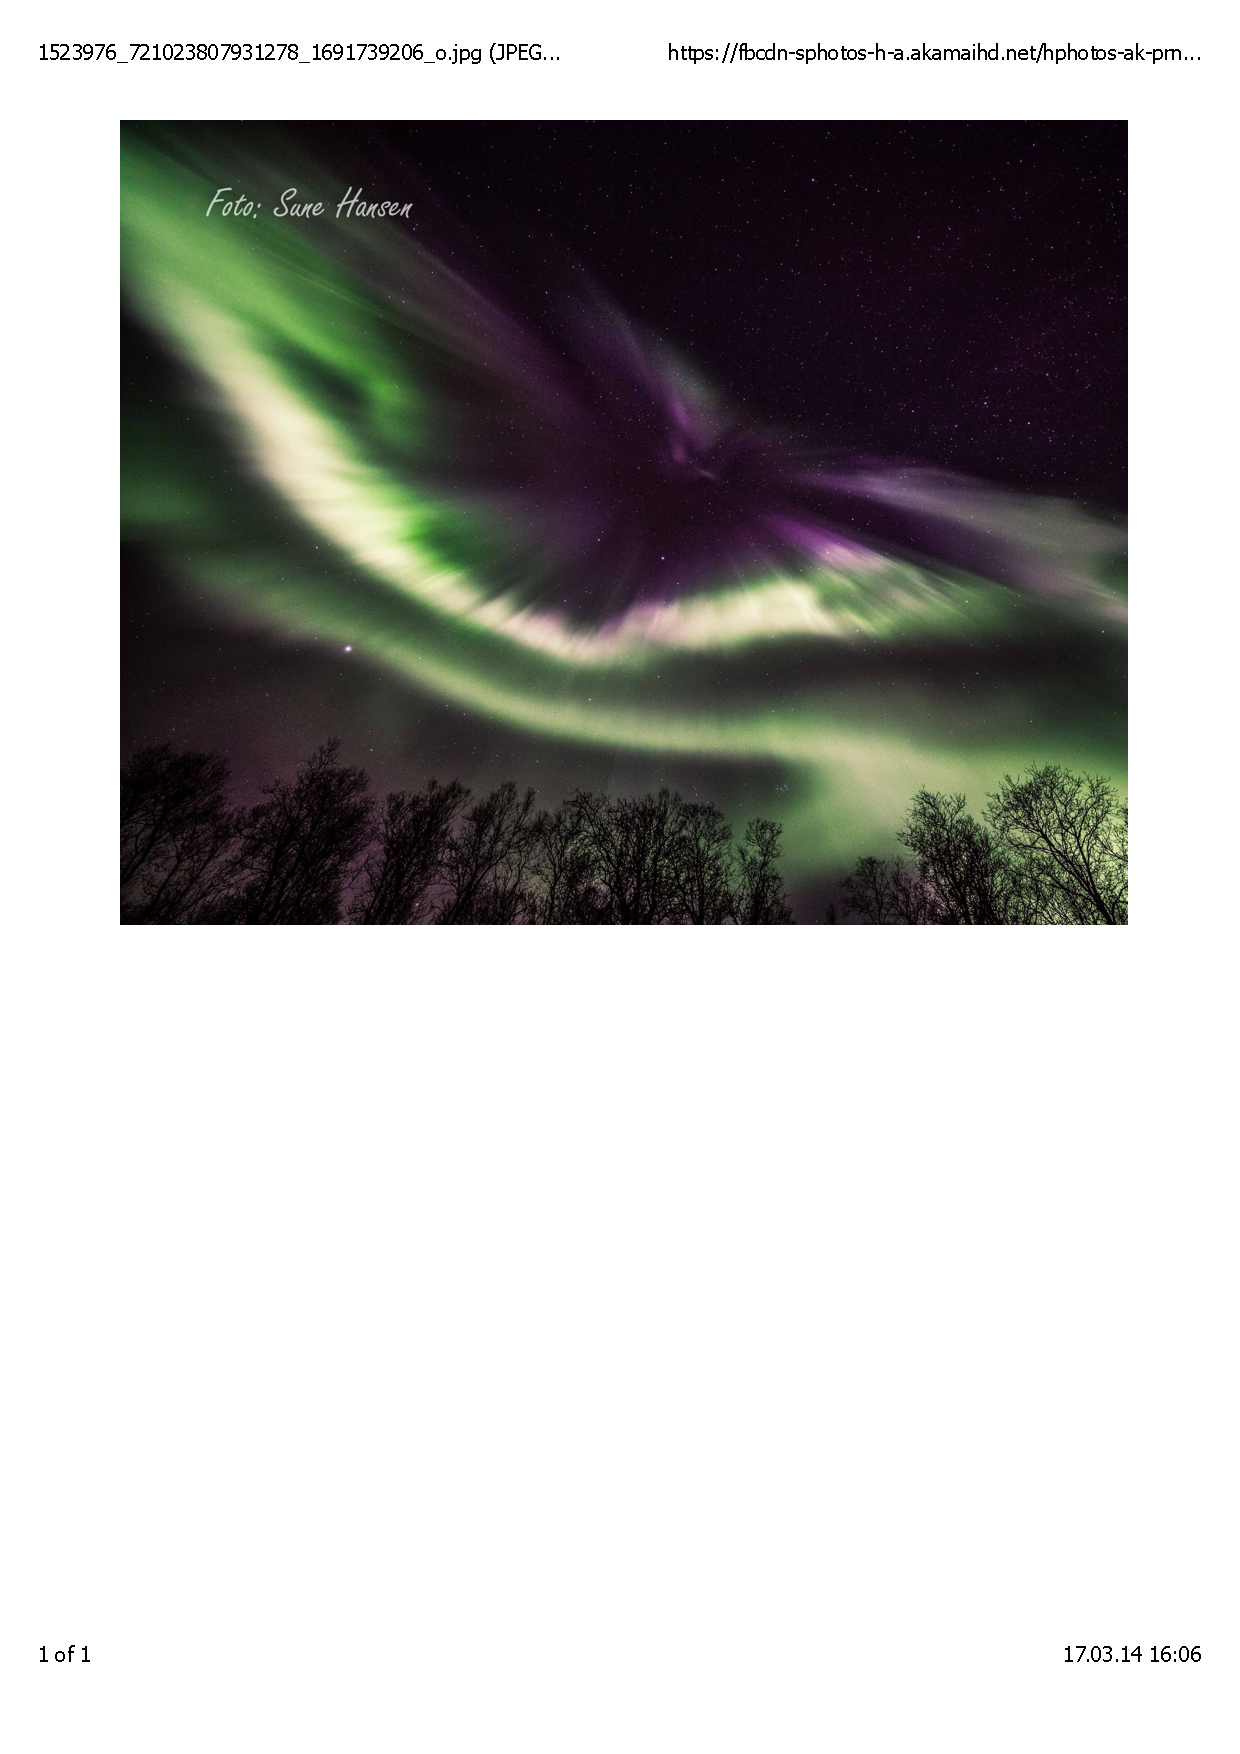
\includegraphics[viewport = 40 400 600 800, clip, scale=0.24]{figures/aurora_2.pdf}
    \end{column}
    \end{columns}
\end{frame}

\begin{frame}
    \frametitle{Summary}
\end{frame}


\end{document}
